\chapter{
Introduction to Bayesian Analysis of GL(M)Ms Using R/WinBUGS
}
\markboth{Chapter 2}{}
\label{chapt.glms}

\vspace{.3in}

%%%% STUFF TO DO 
%%% 1. Prior lack of invariance to transformation stuff: Reference and Figure
%%% 2. Full conditional example from ch. 6 copy notation
%%% 3. Check out algorithm environment
%%% 4. reference for sampling from f() with bounded support
%%% 5. need refs on choosing prior disributions
%%% 6. Check Bayesian p-value definition

A major theme of this book is that spatial capture-recapture models
are, for the most part, just generalized linear models (GLMs) wherein
the covariate, distance between trap and home range center, is
partially or fully unobserved  -- and therefore regarded as 
a random effect. Such models
are usually referred to as Generalized Linear Mixed Models (GLMMs)
and, therefore, SCR models can be thought of as a specialized type of
GLMM. Naturally then, we should consider analysis of these slightly
simpler models in order to gain some experience and, hopefully,
develop a better understanding of spatial capture-recapture models.

In this chapter, we consider classes of GLM models - Poisson and
binomial (i.e., logistic regression) GLMs - that will prove to be
enormously useful in the analysis of capture-recapture models of all
kinds. Many readers are probably familiar with these models because
they represent probably 
the most generally useful models in all of Ecology and, as
such, have received considerable attention in many introductory and
advanced texts. We focus on them here in order to introduce the
readers to the analysis of such models in {\bf R} and {\bf WinBUGS}, 
which we will
translate directly to the analysis of SCR models in subsequent
chapters.  

Bayesian analysis is convenient for analyzing GLMMs because it allows
us to work directly with the conditional model -- i.e., the model that
is conditional on the random effects, using computational methods
known as Markov chain Monte Carlo (MCMC). Learning how to do Bayesian
analysis of GLMs and GLMMs in {\bf WinBUGS} is, in part, the purpose
of this chapter.  While we use {\bf WinBUGS} to do the Bayesian
computations, we organize and summarize our data and execute {\bf
  WinBUGS} from within {\bf R} using the useful package \mbox{\tt
  R2WinBUGS} \citep{sturtz_etal:2005}.  \citet{kery:2010}, and
\citet{kery_schaub:2011} provide excellent introductions to the basics
of Bayesian analysis and GLMs at an accessible level. We don't want to
be too redundant with those books and so we avoid a detailed
treatement of Bayesian methodology - instead just providing a cursory
overview so that we can move on and attack the problems we're most
interested in related to spatial capture-recapture.  In addition,
there are a number of texts that provide general introductions to
Bayesian analysis, MCMC, and their applications in Ecology including
\citet{mccarthy:2007}, \citet{kery:2010}, \citet{link_barker:2009},and
\citet{king_etal:2009}.


While this chapter is about Bayesian analysis of GLMMs, such models
are routinely analyzed using likelihood methods too, as discussed by
\citet{royle_dorazio:2008}, and \citet{kery:2010}. Indeed, likelihood
analysis of such models is the primary focus of many applied
statistics texts, a good one being \citet{zuur_etal:2009}. Later in
this book, we will use likelihood methods to analyze SCR models but,
for now, we concentrate on providing a basic introduction to Bayesian
analysis because that is the approach we will use in a majority of
cases in later chapters.


\section{ Notation}

We will sometimes use conventional ``bracket notation'' to refer to
probability distributions. If $y$ is a random variable the $[y]$
indicates its distribution or its probability density/mass function
(pdf, pmf) depending on context. If $x$ is another random variable
then $[y|x]$ is the conditional distribution of $y$ given $x$, and
$[y,x]$ is the joint distribution of $y$ and $x$. To differentiate
specific distributions in some contexts we might label them $g(y)$,
$g(y|\theta)$, $f(x)$, or similar. We will also write $y \sim
\mbox{Normal}(\mu,\sigma^{2})$ to indicate that $y$ ``is distributed as'' a normal
random variable with parameters $\mu$ and $\sigma^{2}$. The expected value
or mean of a random variable is $E[y] = \mu$ ,and $Var[y] = \sigma^{2}$ is
the variance of $y$.  To indicate specific observations we'll use an
index such as ``$i$''. So, $y_{i}$ for $i=1,2,\ldots,n$ indicates
observations for $n$ individuals. Finally, we write $\Pr(y)$ to indicate specific probabilities, i.e., of events ``$y$'' or similar. 


To illustrate these concepts and notation, suppose $z$ is a binary
outcome (e.g., species occurrence) and we might assume the model: $z
\sim \mbox{Bern}(p)$ for observations.  Under this model $\Pr(z=1) =
\psi$, which is also the expected value $E[z] = \psi$. The variance is
$Var[z] = \psi*(1-\psi)$ and the probability mass function (pmf) is $[z]
= \psi^{z} (1-\psi)^{1-z}$. Sometimes we write $[z|\psi]$ when it is
important to emphasize the conditional dependence of $z$ on $\psi$. As
another example, suppose $y$ is a random variable denoting whether or
not a species is detected if an occupied site is surveyed. In this
case it might be natural to express the pmf of the observations $y$
{\it conditional} on $z$. That is, $[y|z]$. In this case, $[y|z=1]$ is
the conditional pmf of $y$ given that a site is occupied, and it is
natural to assume that $[y|z=1] = \mbox{Bern}(p)$ where $p$ is the
``detection probability'' - the probability that we detect the
species, given that it is present. The model for the observations $y$
is completely specified once we describe the other conditional pmf
$[y|z=0]$. For this conditional distribution it is sometimes
reasonable to assume $\Pr(y=1|z=0) = 0$ (\citet{mackenzie_etal:2002};
see also \citet{royle_link:2006}). That is, if the species is absent,
the probability of detection is 0. This implies that
$\Pr(y=0|z=0)=1$. To allow for situations in which the true state $z$
is unobserved, we  assume that $[z]$ is Bernoulli with parameter
$\psi$.  In this case, the marginal distribution of $y$ is
\[
 [y] = [y|z=1]Pr(z=1) + [y|z=0]Pr(z=0)
\]
because $[y|z=0]$ is a point mass at $y=0$, by assumption, then 
\[
\Pr(y=1) = p \psi
\]
And
\[
\Pr(y=0) = (1-p)*\psi + (1-\psi)
\]


\section{
GLMs and GLMMs}
We have asserted already that SCR models work out most of the time to
be variations of GLMs and GLMMs. Some of you might therefore ask: What
are GLMs and GLMMs, anyhow?   These models are covered extensively in
many very good applied statistics books and we refer the reader
elsewhere for a detailed introduction. We think \citet{kery:2010},
\citet{kery_schaub:2011}, and \citet{zuur_etal:2009} are all
accessible treatments of considerable merit. Here, we'll give the 1
minute 
treatment of GLMMs, not trying to be complete but rather only 
to preserve a coherent organization to the book.


The generalized linear model (GLM) is an extension of standard linear
models by allowing the response
variable to have some distribution from the exponential family of
distributions (i.e., not just normal). This includes the normal
distribution but also dozens of others such as the Poisson, binomial,
gamma, exponential, and many more. In addition, GLMS allow the
response variable to be related to the predictor variables (i.e.,
covariates) using a
link function, which is usually nonlinear.  Finally, GLMs typically
accommodate a relationship between the mean and variance. The
classical reference for GLMs is \citet{nelder_wedderburn:1972} and
also \citet{mccullagh_nelder:1989}.
The GLM consists of three components:
\begin{itemize}
\item[1.] A probability distribution for the dependent variable $y$, 
from a class of probability distributions known as the exponential family.
\item[2.] A ``linear predictor'' $\eta = {\bf X}{\bold \beta}$  . 
\item[3.] A link function $g$ that relates $E[y]$ to the linear predictor, $E[y] = \mu = g^{-1}(\eta)$. Therefore $g(E[y]) = \eta$.
\end{itemize}

The dependent variable $y$ is assumed to be an outcome from a
distribution of the exponential family which includes many common
distributions including the normal, gamma, Poisson, binomial, and many
others. The mean of the distribution of $y$ is assumed to depend on predictor variables $x$ according to 
\[
 g(E[y]) = {\bf x}'{\bold \beta}
\]
where $E[y]$ is the expected value of $y$, and ${\bf x}'{\bold \beta}$
is termed the {\it linear predictor}, i.e., a linear function of the
predictor variables with unknown parameters ${\bold \beta}$ to be
estimated.  The function $g$ is the link function. In standard GLMs,
the variance of $y$ is a function $V$ of the mean of $y$: $Var(y) =
V(\mu)$ (see below for examples).

A Poisson GLM posits that $y \sim \mbox{Poisson}(\lambda)$ with $E[y]
=\lambda$ and usually the model for the mean is specified using the
{\it log link function} by
\[
log(\lambda_{i}) = \beta_0 + \beta_{1}*x_{i}
\]
The variance function is $\mbox{V}(y_{i}) = \lambda_{i}$.  The
binomial GLM posits that $y_{i} \sim \mbox{Binomial}(K,p)$ where $K$
is the fixed sample size parameter and $E[y_{i}] = K*p_{i}$. Usually
the model for the mean is specified using the {\it logit link
  function} according to
\[
 logit(p_{i}) = \beta_{0} + \beta_{1}*x_{i}
\]
Where $logit(u) = log(u/(1-u))$.  The inverse-logit function, $g^{-1}$ ,
is a function we will refer to as ``expit'', so that $expit(u) =
exp(u)/(1+exp(u))$.

A GLMM is the extension of GLMs to accommodate ``random
effects''. Often this involves adding a normal random effect to the
linear predictor, and so a simple example is:
\[
 \log(\lambda_{i}) = \alpha_{i} + \beta_{1}*x_{i}
\]
where
\[
 \alpha_{i} \sim \mbox{Normal}(\mu,\sigma^{2})
\]
%Many other probability distributions and formulations of the linear
%predictor might be considered.  It is not widely appreicated that
%the link function and
%distribution of the random effect interact directly to affect the
%implied probability distribution of the linear predictor. For the
%Poisson case just considered, $\lambda_{i}$ has a log-normal
%distribution. However, if we set $\lambda_{i} = \alpha_{i}exp(\beta*x_{i})$
%where $\alpha_{i}$ has a Gamma distribution, then $\lambda_{i}$ has
%similarly a gamma distribution with modified scale parameter.  These
%different model assumptions are seldom evaluated formally in practice
%although in many practical situations (in ecology), they imply
%specific things about the ecological process being studied 
%(e.g., see \citet{royle_dorazio:2008} section XYZ on occupancy 
%logit/cloglog etc..).



\section{Bayesian Analysis}

Bayesian analysis is unfamiliar to many ecological researchers because
older cohorts of ecologists were largely educated in the classical
statistical paradigm of frequentist inference. But advances in
technology and increasing exposure to benefits of Bayesian analysis
are fast making Bayesians out of people or at least making Bayesian
analysis an acceptable, general, alternative to classical, frequentist
inference.

Conceptually, the main thing about Bayesian inference is that it uses
probability directly to characterize uncertainty about things we don't
know.  ``Things'', in this case, are parameters of models and, just as
it is natural to characterize uncertain outcomes of stochastic
processes using probability, it seems natural also to characterize
information about unknown ``parameters'' using probability. At least
this seems natural to us and, we think, most ecologists either
explicitly adopt that view or tend to fall into that point of view
naturally.  Conversely, frequentists use probability in many different
ways, but never to characterize uncertainty about
parameters\footnote{To hear this will be shocking to some readers
  perhaps.} Instead, frequentists use probability to characterize the
behavior of {\it procedures} such as estimators or confidence
intervals (see below), which can lead to some inelegant or unnatural
interpretations of things.  It is paradoxical that people readily
adopt a philosophy of statistical inference in which the things you
don't know (i.e., parameters) should {\it not} be regarded as random
variables, so that, as a consequence, one cannot use probability to
characterize ones state of knowledge about them.


\subsection{Bayes Rule}

As its name suggests, Bayesian analysis makes use of Bayes' rule in
order to make direct probability statements about model
parameters. Given two random variables $z$ and $y$, Bayes rule relates
the two conditional probability distributions $[z|y]$ and $[y|z]$ by
the relationship:
\[
[z|y] = [y|z][z]/[y]
\]
Bayes' rule itself is a mathematical fact and there is no debate in
the statistical community as to its validity and relevance to many
problems. Generally speaking, these distributions are characterized as
follows: $[y|z]$ is the conditional probability distribution of $y$
{\it given} $z$, $[z]$ is the marginal distribution of $z$ and $[y]$
is the marginal distribution of $y$. In the context of Bayesian
inference we usually associate specific meanings in which $[y|z]$ is
thought of as ``the likelihood'', $[z]$ as the ``prior'' and so on. We
leave this for later because here the focus is on this expression of
Bayes rule as a basic fact of probability. 

As an example of a simple application of Bayes rule,
consider the problem of determining species presence at a sample
location based on imperfect survey information. Let $z$ be a binary
random variable that denotes species presence $(z=1)$ or absence
$(z=0)$, let $\Pr(z=1) = \psi$ where $\psi$ is usually called
occurrence probability, ``occupancy'' \citep{mackenzie_etal:2002} or ``prevalence''. 
Let $y$ be the {\it observed} presence
($y=1$) or absence ($y=0$), and let $p$ be the probability that a
species is detected in a single survey at a site given that it is
present. Thus, $\Pr(y=1|z=1)=p$. The interpretation of this is that,
if the species is present, we will only observe presence with
probability $p$. In addition, we assume here that $\Pr(y=1|z=0) =
0$. That is, the species cannot be detected if it is not present which
is a conventional view adopted in most biological sampling problems (but
see \citet{royle_link:2006}).
If we survey a site $T$ times but never detect the species,
then this clearly does not imply that the species is not present
($z=0$) at this site. Rather, our degree of belief in $z=0$ should be
made with a probabilistic statement
$\Pr(z=1|y_1=0,\ldots,y_{T}=0)$. If the $T$ surveys are independent so
that we might regard $y_{t}$ as $iid$ Bernoulli trials, then the total
number of detections, say $y$, is Binomial with probability $p$ then
we can use Bayes rule to compute the probability that it is present
given that it is not detected in $T$ samples. In words, the expression
we seek is:
\[
\Pr(\mbox{present} | \mbox{not detected}) = \frac{\Pr(\mbox{not detected} |
  \mbox{present})\Pr(\mbox{present})}{\Pr(\mbox{detected})}
\]
Mathematically, this is 
\[
\Pr(z=1|y=0) = \Pr(y=0|z=1)\Pr(z=1)/\Pr(y=0) = 
[(1-p)^{T} \psi]/[ (1-p)^T \psi + (1-\psi) ].
\]
To apply this, 
suppose that $T=2$ surveys are done at a wetland for a species of
frog, and the species is not detected there. Suppose further that $\psi
= .8$ and $p = .5$ are obtained from a prior study.  Then the
probability that the species is present at this site is
$.25*.8/(.25*.8 + .2) = 0.50$. That is, there seems to be about a
50/50 chance that the site is occupied despite the fact that the
species wasn't observed there.

In summary, Bayes' rule provides a simple linkage between the
conditional probabilities $[y|z]$ and $[z|y]$ which is useful whenever
one needs to deduce one from the other. 
Bayes' rule as a basic fact of probability is not disputed. 


\subsection{Bayesian Inference}


What is controversial to some is the scope and manner in which Bayes
rule is applied by Bayesian analysts. Bayesian analysts assert that
Bayes rule is relevant, in general, to all statistical problems by
regarding all unknown quantities of a model as realizations of random
variables - this includes ``data'', latent variables, and also
``parameters''. Classical (non-Bayesian) analysts sometimes object to
regarding ``parameters'' as outcomes of random variables. Classically,
parameters are thought of as ``fixed but unknown'' (using the
terminology of classical statistics). Of course, in Bayesian analysis
they are also unknown and, in fact, there is a single data-generating
value and so they are also fixed. The difference is that this fixed
but unknown value is regarded as having been generated from some
probability distribution. Specification of that probability
distribution is necessary to carryout Bayesian analysis, but it is not
required in classical frequentist inference. 


To see the general relevance of Bayes rule in the context of
statistical inference, let $y$ denote observations - i.e., ``data'' -
and let $[y|\theta]$ be the observation model (often colloquially
referred to as the ``likelihood'').  Suppose theta is a parameter of
interest having (prior) probability distribution $[\theta]$. These are
combined to obtain the posterior distribution using Bayes' rule, which
is:
\[
 [\theta|y]= [y|\theta][\theta]/[y]
\]
Asserting the general relevance of Bayes rule to all statistical
problems, we can conclude that the two main features of Bayesian
inference are that: (1) ``parameters'' $\theta$ are regarded as realizations of
a random variable and, as a result, (2) inference is based on the
probability distribution of the parameters given the data,
$[\theta|y]$,
which is
called the posterior distribution. This is the result of using Bayes
rule to combine ``the likelihood'' and the prior distribution.  The
key concept is regarding parameters as realizations of a random
variable because, once you admit this conceptual view, this leads
directly to the posterior distribution, a very natural quantity upon
which to base inference about things we don't know -  including
parameters of statistical models.  In particular, $[\theta|y]$ is a
probability distribution for $\theta$ and therefore we can make direct
probability statements to characterize uncertainty about
$\theta$. 

The denominator of our invocation of Bayes rule, $[y]$,
is the marginal distribution of the data $y$.  We note without further
remark right now that, in many practical problems, this can be an
enormous pain to compute. The main reason that the Bayesian paradigm
has become so popular in the last 20 years or so is because methods
exist for characterizing the posterior distribution that do not
require that we possess a mathematical understanding of $[y]$, i.e.,
we never have to compute it or know what it looks like, or know
anything specific about it.

A common misunderstanding on the distinction between Bayesian and
frequentist inference goes something like this ``in frequentist
inference parameters are fixed but unknown but in a Bayesian analysis
parameters are random.'' At best this is a sad caricature of the
distinction and at worst it is downright wrong. What is true is that,
to a Bayesian, parameters are random variables. However, a Bayesian
assumes, just like a frequentist, that there was a single
data-generating value of that parameter - a fixed, and unknown value
that produced the given data set.
The distinction between Bayesian and frequentist approaches is that
Bayesians regard the parameter as a random variable, and its value as
the outcome of a random value, on par with the observations. This
allows Bayesians to use probability to make direct probability
statements about parameters. Frequentist inference procedures do not
permit direct probability statements to be made about parameter
values -- because parameters are not random variables!

While we can understand the conceptual basis of Bayesian inference
merely by understanding Bayes rule -- that's really all there is to it
-- it is not so easy to understand the basis of classical
``frequentist'' inference which is mostly
like\footnote{Characterization from Sims REF XYZ} a ``basket of
methods'' with little coherent organization. What is mostly coherent
in frequentist inference is the manner in which items in this basket
of methods are evaluated -- the performance of a given procedure is
evaluated by ``averaging over'' hypothetical realizations of $y$,
regarding the {\it estimator} as a random variable. For example, if
$\hat{\theta}$ is an estimator of $\theta$ then the frequentist is
interested in $E_{y}[\hat{\theta}|y]$ which is used to characterize
bias. If the expected value of $\hat{\theta}$, when averaged over
realizations of $y$, is equal to $\theta$, then $\hat{\theta}$ is
unbiased. 

The view of parameters as fixed constants and estimators as random variables
leads to interpretations that are not so straightforward. For
example confidence intervals having the interpretation ``95\%
probability that the interval contains the true value" and p-values
being "the probability of observing an outcome as extreme or more than
the one observed.'' These are far from intuitive interpretations to
most people.  Moreover, this is conceptually probblematic to some
because the hypothetical realizations that characterize the
performance of our procedure we will never get to observe.

While we do tend to favor Bayesian inference for the conceptual
simplicity (parameters are random, posterior inference), we mostly
advocate for a pragamatic non-partisian approach to inference because,
frankly, some of these ``bucket of methods'' are actually very
convenient in certain situations as we will see in later chapters.


\subsection{Prior distributions}


The prior distribution $[\theta]$ is an important feature of Bayesian
inference. As a conceptual matter, 
the prior distribution characterizes ``prior beliefs'' or ``prior
information'' about a parameter. Indeed, 
an oft-touted benefit of Bayesian analysis is the ease with which
prior information can be included in an analysis.
However, more commonly, the prior is chosen to
express a lack of prior information, even if previous studies have
been done and even if the investigator does in fact know quite a bit
about a parameter. 
This is because 
the manner in which prior information is embodied in a prior (and the
amount of information) is 
usually very subjective and thus the result can wind up being very
contentious, e.g., if different investigators might report different
results based on subjective assessments of things. Thus it is usually
better to ``let the data speak'' and use priors that reflect absence
of information beyond the data set being analyzed. 

But still the need occasionally arises to embody prior information or
beliefs about a parameter formally into the estimation scheme.
 In SCR models we often have a parameter that is closely linked
to ``home range radius'' and thus auxiliary information on the home
range size of a species can be used as prior information (e.g., see
\citet{chandler_royle:2012} ; also chapter XYZ). 

XXXXXXXX

noninformative prior on one scale is informative on another scale.
e.g., flat prior on logit(p) is very different from uniform(0,1) on
p...
show graphic......

reference to non-invariance of prior distributions to transformation......

XXXXXXXX

\subsection{Posterior Inference}

In Bayesian inference, we are not focusing on estimating a single
point or interval but rather on characterizing a whole distribution --
the posterior distribution -- from which one can report any summary of
interest. A point estimate might be the posterior mean, median, mode,
etc..  In many applications in this book, we will compute 95\%
Bayesian intervals using the 2.5\% and 97.5\% quantiles of the
posterior distribution. For such intervals, it is correct to say
$\Pr(L < \theta < U) = 0.95$. That is, "the probability that $\theta$
is between $L$ and $U$ is $0.95$". It is not a subtle thing that this
cannot be said using frequentist methods - although people tend to say
it anyway and not really understand why it is wrong or even that it is
wrong. This is actually a failing of frequentist ideas and the
inability of frequentists to get people to overcome their natural
tendency to use probability - which is something that, as a
frequentist, you simply cannot do in the manner that you would like
to.



Posterior inference is the main practical element of Bayesian
analysis. We get to make an inference conditional on the data that we
actually observed - i.e., what we actually know.  To us, this seems
logical - to condition on what we know. Conversely, frequentist
inference is based on considering average performance over
hypothetical unobserved data sets (i.e., the ``relative frequency''
interpretation of probability).  Frequentists know that their
procedures work well when averaged over all hypothetical, unobserved,
data sets but no one ever really knows how well they work for the
specific data set analyzed. That seems like a relevant question to
biologists who oftentimes only have their one, extremely valuable,
data set.  This distinction comes into play a lot in exposing
philosophical biases in the peer review of statistical analyses in
ecology in the sense that, despite these opposing conceptual views to
inference (i.e. conditional on the data you have, or averaged over
hypothetical realizations), those who conduct a Bayesian analysis are
often (in ecology, almost always) required to provide a frequentist
evaluation of their Bayesian procedure.

\subsection{Small sample inference}

Using Bayesian inference, we obtain an estimate of the posterior
distribution which is an exhaustive summary of the state-of-knowledge
about an unknown quantity. It is the posterior distribution - not an
estimate of that thing. It is also not, usually, an approximation
except to within Monte Carlo error (in cases where we use simulation
to calculate it).  One of the great virtues of Bayesian analysis which
is not really appreciated is that it is completely valid for any
particular sample size. i.e., it is $[\theta|y]$, as precise as we
claim it to be based on our ability to do calculations, for the
particular sample size and observations that we have even if we have
only a single datum $y$.  The same cannot be said for almost all
frequentist procedures in which estimates or variances are very often
(almost always in practice) based on ``asymptotic approximations'' to
the procedure which is actually being employed.

There seems to be a prevailing view in statistical ecology that
classical likelihood-based procedures are virtuous because of the
availability of simple formulas and procedures for carrying out
inference, such as calculating standard errors, doing model selection
by AIC, and assessing goodness-of-fit.  In large samples, this may be
an important practical benefit, but the theoretical validity of these
procedures cannot be asserted in most situations involving small
samples.  This is not a minor issue because it is typical in many
wildlife sampling problems - especially in surveys of carnivores or
rare/endangered species - to wind up with a small, sometimes extremely
small, data set. For example, a recent paper on the fossa
(Cryptoprocta ferox), an endangered carnivore in Madagascar, estimated
an adult density of 0.18 adults / km sq based on 20 animals captured
over 3 years \citep{hawkins_racey:2005}. A similar paper on the
endangered southern river otter (Lontra provocax) estimated a density
of 0.25 animals per river km based on 12 individuals captured over 3
years \citep{sepulveda_etal:2007}. \citet{gardner_etal:2010} analyzed
data from a study of the Pampas cat, a species for which very little
is known, wherein only 22 individual cats were captured .during the
two year period.  \citet{trolle_kery:2005} reported only 9 individual
ocelots captured and \citet{jackson_etal:2006} captured 6 individual
snow leopards using camera trapping. Thus, studies of rare and/or
secretive carnivores necessarily and flagrantly violate one of Le
Cam's Basic Principles, that of ``If you need to use asymptotic
arguments, do not forget to let your number of observations tend to
infinity.''\citep{lecam:1990}.

The biologist thus faces a dilemma with such data. On one hand, these
datasets, and the resulting inference, are often criticized as being
poor and unreliable. Or, even worse\footnote{Actual quote from a
  referee}, ``the data set is so small, this is a poor analysis.''  On
the other hand, such data may be all that is available for species
that are extraordinarily important for conservation and management.
The Bayesian framework for inference provides a valid, rigorous, and
flexible framework that is theoretically justifiable in arbitrary
sample sizes. This is not to say that one will obtain precise
estimates of density or other parameters, just that your inference is
coherent and justifiable from a conceptual and technical statistical
point of view. That is, we report the posterior probability
$\Pr(D|data)$ which is easily interpretable and just what it is
advertised to be and we don't need to do a simulation study to
evaluate how well some approximate $\Pr(D|data)$ deviates from the
actual $\Pr(D|data)$ because they are precisely the same quantity.



\section{Characterizing posterior distributions by MCMC simulation}  

In practice, it is not really feasible to ever compute the marginal
probability distribution $\Pr(y)$, the denominator resulting from
application of Bayes' rule. For decades this impeded the adoption of
Bayesian methods by practitioners. Or, the few Bayesian analyses done
were based on asymptotic normal approximations to the posterior
distribution. While this was useful stuff from a theoretical and
technical standpoint and, practically, it allowed people to make the
probability statements that they naturally would like to make, it was
kind of a bad joke around the Bayesian water-cooler to, on one hand,
criticize classical statistics for being, essentially, completely ad
hoc in their approach to things but then, on the other hand, have to
devise various approximations to what they were trying to
characterize. The advent of Markov chain Monte Carlo (MCMC) methods
has made it easier to calculate posterior distributions for just about
any problem to arbitrary levels of precision.

Broadly speaking, MCMC is a class of methods for drawing random
numbers (sampling or simulating) from the target posterior
distribution.  Thus, even though we might not recognize the posterior
as a named distribution or be able to analyze its features
analytically, e.g., devise mathematical expressions for the mean and
variance, we can use these MCMC methods to obtain a large sample from
the posterior and then use that sample to characterize features of the
posterior. What we do with the sample depends on our intentions --
typically we obtain the mean or median for use as a point estimate,
and take a confidence interval based on Monte Carlo estimates of the
quantiles.  These are estimates, but not like frequentist
estimates. Rather, they are Monte Carlo estimates with an associated
Monte Carlo error which is largely determined arbitrarily by the
analyst. They are not estimates qualified by a sampling distribution
as in classical statistics. If we run our MCMC long enough then our
reported value of $E[\theta|y]$ or any feature of the posterior
distribution is precisely what we say it is. There is no ``sampling
variation'' in the frequentist sense of the word.  In summary, the
MCMC samples provide a Monte Carlo characterization of {\it the}
posterior distribution.


\section{What Goes on Under the MCMC Hood}

We will develop and apply MCMC methods in some detail for spatial
capture-recapture models in chapter \ref{chapt.mcmc}. Here we provide
a simple illustration of some basic ideas related to the practice of MCMC.

A type of MCMC method relevant to most problems is Gibbs sampling (REF
XYZ XYZ),
which is based on the idea of iterative simulation from the ``full
conditional'' distributions (also called conditional posterior
distributions). The full conditional distribution for an unknown
quantity is the conditional distribution of that quantity given every
other random variable in the model - the data and all other
parameters. For example, for a normal regression model with $y \sim
\mbox{Normal}(\alpha + \beta x , 1)$ then the two full conditionals are, in
symbolic terms,
\[ 
[\alpha|y,\beta]
\]
 and 
\[
[\beta|y,\alpha].
\]
We might use our knowledge of probability to identify these
mathematically. In particular, by Bayes' Rule, $[\alpha|y,\beta] =
[y|\alpha,\beta][\alpha|\beta]/[y|\beta]$ and similarly for
$[\beta|y,\alpha]$. For example, if we have priors for $[\alpha]$ and $[\beta]$
which are also normal distributions, some algebra reveals that
XXXX COPY NOTATION FFROM CH. 6 XXXXX
\[
[\alpha|y,\beta] = Normal(ybar,...weighted variance here...). 
\]
Similarly,
\[
 [\beta|y,\alpha] is normal(........) 
\]

The MCMC algorithm for this model has us simulate in succession,
repeatedly, from those two distributions. See \citet{gelman_etal:2004}
for more examples of Gibbs sampling for the normal model. A
conceptual representation of the MCMC algorithm for this simple model
is therefore:
XXXX Check out ALGORITHM environment XXXXX
\begin{verbatim}
 Algorithm

       0. Initialize $\alpha$ and $\beta$

       Repeat{
           1. Draw a new value of $\alpha$ from Eq. \ref{xyz}

           2. Draw a new value of $\beta$ from Eq. \ref{xyz}
       }
\end{verbatim}

As we just saw for this simple ``normal-normal'' model it is sometimes
possible to specify the full conditional distributions
analytically. In general, when certain so-called conjugate prior
distributions are chosen, the form of full conditional distributions
is similar to that of the observation model. In this normal-normal
case, the normal distribution for the mean parameters is the conjugate
prior under the normal model, and thus the full-conditional
distributions are also normal. This is convenient because, in such
cases, we can simulate directly from them using standard methods (or
{\bf R}
functions).  But, in practice, we don't really ever need to know such
things because most of the time we can get by using a simple
algorithm, called the Metropolis-Hastings (henceforth ``MH'')
algorithm, to obtain samples from these full conditional distributions
without having to recognize them as specific, named, distributions. 
This gives us enormous freedom in developing models
and analyzing them without having to resolve them mathematically
because to implement the MH algorithm we need only identify the full
conditional distribution up to a constant of proportionality, that
being the marginal distribution in the denominator (e.g., $[y|\beta]$
above).

We will talk about the Metropolis-Hastings algorithm shortly, and we
will use it extensively in the analysis of SCR models (e.g., chapter
\ref{chapt.mcmc}). 

\subsection{Rules for constructing full conditional distributions}  
\label{glms.sec.rules}

The basic strategy for constructing full-conditional distributions for
devising MCMC algorithms can be reduced conceptually to a couple of
basic steps summarized as follows:
\begin{itemize}
\item[(step 1)] Collect all stochastic components of the model; 
\item[(step 2)] Recognize and express the full conditional in question
  as proportional to the product of all components;
\item[(step 3)] Remove the ones that don't have the focal parameter in them. 
\item[(step 4)] Do some algebra on the result in order to identify the resulting pdf or pmf. 
\end{itemize}
Of the 4 steps, the last of those is the main step that requires quite
a bit of statistical experience and intuition because various
algebraic tricks can be used to reshape the mess into something
noticeable - i.e., a standard, named distribution. But step 4 is not
necessary if we decide instead to use the Metrpolis-Hastings algorithm
as described below.

To illustrate for computing $[\alpha|y,\beta]$ we first apply step 1
and identify the model components as: $[y|\alpha, \beta]$, $[\alpha]$
and $[\beta]$. Step 2 has us write $[\alpha|y,\beta] \propto
[y|\alpha,\beta][\alpha][\beta]$.  Step 3: We note that $[\beta]$ is not a
function of alpha and therefore we remove it to obtain $[\alpha|y,\beta]
\propto [y|\alpha,\beta][\alpha]$. Similarly we obtain $[\beta|y,\alpha]
\propto [y|\alpha,\beta][\beta]$. We apply step 4 and manipulate
these algebraically to arrive at the result or, alternatively, we can
sample them indirectly using the Metropolis-Hastings algorithm (see
below).


\subsection{Metropolis-Hastings algorithm}
 
The Metropolis-Hastings (MH) algorithm is a completely generic method for
sampling from any distribution, say $f(\theta)$. In our applications,
$f(\theta)$ will typically be the full conditional distribution of
$\theta$. 
While we sometimes use Gibbs sampling, we seldom
use ``pure'' Gibbs sampling because we might use MH to sample from one
or more of the full conditional distributions.
When the MH algorithm is used to sample from  full
conditional distributions of a Gibbs sampler the resulting hybrid algorithm is
called 
 {\it Metrpolized Gibbs sampling} or
more commonly {\it Metropolis-within-Gibbs}.
Shortly we will
actually construct such an algorithm for a simple class of models.

The MH algorithm generates candidates from some
proposal or candidate-generating distribution, that may be conditional
on the current value of the parameter, denoted by
$h(\theta^{*}|\theta^{t})$. Here, $\theta^{*}$ is the {\it candidate}
or proposed 
value and $\theta^{t}$ is the current value, i.e., at iteration $t$ of
the MCMC algorithm.  The proposed value
is accepted with probability
XXXX check notation with Rahel XXXXXX
\[
r = \frac{ f(\theta^{*}) h(\theta^{t}|\theta^{*})}
    {f(\theta^{t}) h(\theta^{*}|\theta^{t}) }
\]
which we call the MH acceptance probability. 
This ratio can sometimes be $>1$ in which case we set it equal to
1. It is useful to note that $h()$ can be anything at all. Absolutely
anything!  You can generate candidate values from a $normal(0,1)$
distribution, from a uniform(-3455,3455) distribution, or anything of
proper support.  Note, however, that good choices of $h()$ are those
that approximate the posterior distribution. Obviously if $h() =
f(\theta|y)$ (i.e., the posterior) then you always accept the draw,
and it stands to reason that proposals that are more similar to
$f(\theta|y)$ will lead to higher acceptance probabilities. No matter
the choice of $h()$, we can evaluate this ratio numerically because
the marginal $f(y)$ cancels from both the numerator and
denominator, which is the magic of the MH algorithm.


A special kind of $h()$ are those that are symmetric, which means that
$h(a|b) = h(b|a)$ in which case $h(a|b)$ and $h(b|a)$ just cancel
out from the MH acceptance probability and $r$ is then just the ratio
of the target density evaluated at the candidate value to that
evaluated at the current value. 
A type of symmetric proposal useful in many situations is the
so-called {\it random-walk} proposal distribution where candidate values
are drawn from a normal distribution with mean equal to the current
value and some standard deviation, say $\delta$, which is prescribed by
the user. For parameters that have support on the real line, e.g., $\alpha$
in our example above, the random walk proposal generator has us
generate $\alpha^{*} \sim \mbox{Normal}(\alpha^{t},\delta)$.  If we set $\delta$
very small we have a high probability of accepting the proposal and
vice versa.  In practice, we ``tune'' delta to achieve a compromise
between acceptance rate and efficient mixing of the Markov chains (see below for an
example) normally assessed by autocorrelation. Low $\delta$ increases
the acceptance rate but will tend to produce Markov chains with high
autocorrelation, and vice versa. 

{\bf Parameters with bounded support}: Many models contain parameters that
have  bounded support. E.g., variance parameters live on $[0,\infty]$,
parameters that represent probabilities live on $[0,1]$, etc..
 In that case it is sometimes convenient to use a random
walk proposal distribution that can generate any real number (e.g., a
normal random walk proposal). In that case, 
we can just reject parameters that are
outside of the parameter space (XXXX REF FOR THIS XXXX). 



\section{Practical Bayesian Analysis and MCMC}

There are a number of really important practical issues to be
considered in any Bayesian analysis and we cover some of these briefly
here.

\subsection{Choice of prior distributions} 

{\bf XXX integrate this material with previous section on prior
distributions XXXXXX}

Bayesian analysis requires that we choose prior
distributions for all of the structural parameters of the model (we
use the term structural parameter to mean all parameters that aren't
customary thought of as latent variables). We will strive to use
priors that are meant to express little or no prior information -
default or customary ``non-informative'' or diffuse priors. This will
be $\mbox{Unif}(a,b)$ priors for parameters that have a natural
bounded support and, for parameters that live on the real line we use
either (1) diffuse normal priors; (2) ``improper'' uniform priors or
(3) sometimes even a bounded $\mbox{Unif}(a,b)$ prior if that greatly
improves the performance of {\bf WinBUGS} or other software doing the MCMC
for us.  In {\bf WinBUGS} a prior with low ``precision'', $\tau$, where
$\tau = 1/\sigma^2$, such as $\mbox{Norm}(0,.01)$ will typically be
used. Of course $\tau = 0.01$ ($\sigma^{2} = 100$) might be very
informative for a regression parameter that has a high
variance. Therefore, we recommend that predictor variables {\it
  always} be standardized. Clearly there are a lot of choices for
ostensibly non-informative priors, and the degree of
non-informativeness depends on the parameterization. For example, a
natural non-informative prior for the intercept of a logistic
regression
\[
\mbox{logit}(p_{i}) = \alpha + \beta x_{i}
\]
Would be $[\alpha] = \mbox{const}$ which is the same as saying $a \sim
Unif(\infty,infty)$, the customary improper uniform prior.
However, we might also use a prior on the parameter $p0
= logit^{-1}(a)$, which is $Pr(y=1)$ for the value $x=0$. Since $p0$ is a
probability a natural choice is $p0 \sim Unif(0,1)$. These two priors can
affect results (see Chapter 3.XYZ), yet they are both sensible
non-informative priors. Choice of priors and parameterization is
very much problem-specific and often largely subjective. Moreover, it
also affects the behavior of MCMC algorithms and therefore the analyst
needs to pay some attention to this issue and possibly try different
things out. 
XXX REFS on prior distributions XXXXXX

\subsection{Convergence and so-forth}

Once we have carried-out an analysis by MCMC, there are many other
practical issues that we have to confront.  One of the most important
is ``have the chains converged?'' Most MCMC algorithms only guarantee
that, eventually, the samples being generated will be from the target
posterior distribution. So-called ``convergence'' of the Markov chain
is achieved when that happens.  Typically a period of transience is
observed in the early part of the MCMC algorithm, and this is usually
discarded as the ``burn-in'' period.

The quick diagnostic to whether convergence has been achieved is that
your Markov chains look ``grassy'' -- see Fig.  \ref{glms.fig.grassy}
below.  Another way to check
convergence is to update the parameters some more and see if the
posterior changes. It is good to confirm convergence using the
``R-hat'' statistic ($\hat{R}$) or Brooks-Gelman-Rubin statistic
\citep{gelman_etal:1996}) which should be close to 1 if the Markov
chains have converged and sufficient posterior samples have been
obtained. In practice, $\hat{R} = 1.2$ is probably good enough for
some problems.  For some models you can't actually realize a low
$\hat{R}$. E.g., if the posterior is a discrete mixture of distributions
then you can be misled into thinking that your Markov chains
have not converged when in fact the chains are just jumping back and
forth in the posterior state-space. So, for example, using model
selection methods (section XYZ) sometimes suggests non-convergence.
Another situation is when one of the parameters is on the boundary of
the parameter space which might appear to be very poor mixing, but all
within some extreme region of the parameter space.\footnote{it would
  be nice if we could compile examples of this later in the book and
  reference back to this point}.
This
kind of stuff is normally ok and you need to think really hard about
the context of the model and the problem before you conclude that your
MCMC algorithm is ill-behaved.

Some models exhibit ``poor mixing'' of the Markov chains or what
people might also say ``have not coverged'' (or ``slow convergence'')
which is a term we would disagree with because the samples might well
be from the posterior (i.e., the Markov chains have converged to the
proper stationary distribution) but simply mix around the posterior
rather slowly. Anyway, poor mixing can happen for a huge number of
reasons -- when parameters are highly correlated (even confounded), or
barely identified from the data, or the algorithms are very terrible
and probably many other reasons.  Slow mixing equates to high
autocorrelation in the Markov chain - the successive draws are highly
correlated, and thus we need to run the MCMC algorithm much longer to
get an effective sample size that is sufficient for estimation - or to
reduce the MC error to a tolerable level.  A strategy often used to
reduce autocorrelation is ``thinning'' - i.e., keep every $m^{th}$
value of the Markov chain output. However, thinning is necessarily
inefficient from the stand point of inference - you can always get
more precise posterior estimates by using all of the MCMC output
regardless of the level of autocorrelation
\citep{maceachern_berliner:1994}. Practical considerations might
necessitate thinning, even though it is statistically inefficient. For
example, in models with many parameters or other unknowns being
tabulated, the output files might be enormous and unwieldy to work
with. In such cases, thinning is perfectly reasonable. In many cases,
how well the Markov chains mix is strongly influenced by
parameterization, standardization of covariates, and the prior
distributions being used. Some things work better than others, and the
investigator should experiment with different settings and 
remain calm when things don't work out perfectly. MCMC is an
art, and a science.


{\bf Is the posterior sample large enough?}  A good rule
of thumb is that you should never report
MCMC results to more than 2 decimal places - because they will always
be different! Look at the MC error which is printed by default in
summaries of BUGS output.  You want that to be smallish relative to the
magnitude of the parameter and this might depend on the purpose of the
analysis. For a preliminary analysis you might settle for a few
percent whereas for a final analysis then certainly less than 1\% is
called for, but you can run 
your MCMC
algorithm as long as it takes. Note that MC error in summaries of the
posterior is not the same as having an ``approximate'' solution in a
standard likelihood analysis or similar.  The approximate SE in
likelihood inference is actually wrong in its actual value.... XYZ.


\subsection{Bayesian confidence intervals} 

The 95\% Bayesian interval based on percentiles of the posterior
is not a unique interval - there are many of them - and the so-called
``highest posterior density'' (HPD) interval is the narrowest
interval. We might compute that frequently because it is easy to do
with an integer parameter which $N$ is (See the next chapter). The
95 \% HPD is not often exactly 95\% but usually slightly more
conservative than nominal because it is the narrowest interval that
contains at least 95\%  of the posterior mass.

\subsection{Estimating functions of parameters}

A benefit of analysis by MCMC is that we can seamlessly estimate
functions of parameters by simply tabulating the desired function of
the simulated posterior draws. For example, if $\theta$ is the
parameter of interest and let $\theta^{(i)}$ for $i=1,2,\ldots,M$ be
the posterior samples of $\theta$. Let $\eta = exp(\theta)$, then a
posterior sample of $\eta$ can be obtained simply by computing
$exp(\theta^{(i)})$ for $i=1,2,\ldots,M$. We give another example in
section 
\ref{glms.sec.xopt}
below and throughout this book.
Almost all SCR models in this book involve at least 1 derived
parameter. For example, density $D$ is a derived parameter, being a
function of population size $N$ and the area $A$ of the underlying
state-space of the point process (see chapter \ref{chapt.scr0}). 

\section{Bayesian Analysis using WinBUGS}

We won't be too concerned with devising our own MCMC algorithms for
every analysis
although we will do that a few times for fun.  More often, we
will rely on the freely available software package {\bf WinBUGS} or
{\bf JAGS}
for doing this.  We will always execute these {\bf BUGS} engines from
within {\bf R} using the \mbox{\tt R2WinBUGS} (REF XYZ XYZ) or
\mbox{\tt rjags} pacages. {\bf WinBUGS} and {\bf JAGS} are  MCMC black boxes
that takes a pseudo-code description (i.e., written in the {\bf BUGS}
language) of all of the relevant stochastic
and deterministic elements of a model and generates an MCMC algorithm
for that model. But you never get to see the algorithm. Instead,
{\bf WinBUGS}/{\bf JAGS} will run the algorithm and just return the Markov chain output
- the posterior samples of model parameters. 

The great thing about using the {\bf BUGS} language is that it forces
you to become intimate with your statistical model - you have to write
each element of the model down, admit (explicitly) all of the various
assumptions, understand what the actual probability assumptions are
and how data relate to latent variables and data and latent variables
relate to parameters, and how parameters relate to one another. 

While we normally use
{\bf WinBUGS} or {\bf JAGS} in this book, we note that {\bf
 OpenBUGS} is the current active development tree of the {\bf BUGS}
language. See \citet[][ch.xyz]{kery:2010} and 
\citet[][appendix xyz]{kery_schaub:2011} for more on practial analysis
in {\bf WinBUGS}.
That book should also be consulted
for a more comprehensive introduction to using {\bf WinBUGS}. In this
example, we're going to accelerate pretty fast.

\subsection{Linear Regression in WinBUGS}

We provide a brief introductory example of a normal regression model
using a small simulated data set. The following commands are executed
from within your R workspace, the command line being indicated by
\mbox{\tt ``>''}. First, simulate a covariate $x$ and observations $y$ having
prescribed intercept, slope and variance:
\begin{verbatim}
> x<-rnorm(10)
> mu<- -3.2+ 1.5*x
> y<-rnorm(10,mu,sd=4)
\end{verbatim}
The {\bf BUGS} model specification for a normal regression model is
written within {\bf R} as a character string input to the command
\mbox{\tt cat()} and
then dumped to a text file named \mbox{\tt normal.txt}:
\begin{verbatim}
> cat("
model {
   for (i in 1:10){
      y[i]~dnorm(mu[i],tau)        # the "likelihood"
      mu[i]<- beta0 + beta1*x[i]   # the linear predictor
     }
   beta0~dnorm(0,.01)              # prior distributions
   beta1~dnorm(0,.01)
   sigma~dunif(0,100)               
   tau<-1/(sigma*sigma)            # tau is a derived parameter
}
",file="normal.txt")
\end{verbatim}
Alternatively, you
can write the model specifications directly within a text file and
save it in your current working directory, but we do not usually take
that approach in this book.

{\bf Remarks:} {\bf 1.} {\bf WinBUGS} parameterizes the normal in
terms of the mean and inverse-variance, called the precision. Thus,
\mbox{\tt dnorm(0,.01)} implies a variance of 100; 
{\bf 2.} We typically use diffuse normal priors for mean parameters, $\beta_0$ and $\beta_1$ in this case, but sometimes we might use uniform priors with suitable bounds -B and +B.
{\bf 3.} We typically use a $\mbox{Unif}(0,B)$ prior on standard
deviation parameters 
(Gelman XXX 2006 XXXX). But sometimes we might use a gamma prior on the precision parameter $\tau$.
{\bf 4.} In a {\bf WinBUGS} model file, every variable referenced in
the model description has to be
either data, which will be input (see below), a random variable which
must have a probability distribution associated with it using the
``\verb#~#'', or it has to be a derived parameter connected to variables and
data using ``\mbox{\tt <-}''.


To fit the model, we need to describe various data objects to {\bf
  WinBUGS}. In particular, 
we create an {\bf R} list object called \mbox{\tt data} which
are the data objects identified in the BUGS model file.
 In the example, the 
data consist of two objects which exist as $y$ and $x$ in the {\bf R}
workspace and also in the {\bf WinBUGS} model definition. 
 We also have to create an {\bf R} function
that produces a list of starting values \mbox{\tt inits} that get sent to
{\bf WinBUGS}.
 Finally, we identify
the names of the parameters (labeled correspondingly in the {\bf WinBUGS}
model specification) that we want {\bf WinBUGS} to save the MCMC output
for. In this example, we will ``monitor'' the parameters 
$\beta_0$, $\beta_1$, $\sigma$ and $\tau$. 
{\bf WinBUGS} is executed using the {\bf R} command
\mbox{\tt bugs()}.
We set the option \mbox{\tt debug=TRUE} if we want the {\bf WinBUGS}
GUI to stay open (useful for analyzing MCMC output and looking at the
{\bf WinBUGS} error log). Also, we set \mbox{\tt working.dir=getwd()}
so that {\bf WinBUGS} output files and the log file are saved in the
current {\bf R} working directory.  
  All of these activities look like this:
{\small 
\begin{verbatim}
 library("R2WinBUGS")    # "attach" the R2WinBUGS library
 data <- list ( "y","x")
 inits <- function()
  list ( beta1=rnorm(1),beta0=rnorm(1),sigma=runif(1,0,2) )
 parameters <- c("beta0","beta1","sigma","tau")
 out<-bugs (data, inits, parameters, "normal.txt", n.thin=2, n.chains=2, 
             n.burnin=2000, n.iter=6000, debug=TRUE,working.dir=getwd())
\end{verbatim}
}

{\bf Remarks:} A common question is ``how should my data be
formatted?'' That depends on how you describe the model in the {\bf
  BUGS} language, how your data are input into {\bf R} and
subsequently formatted.  There is no unique way to describe any
particular model and so you have some flexibility. We talk about data
format further in the context of capture-recapture models and SCR
models in chapter \ref{chapt.scr0} and elsewhere.  In general,
starting values are optional but we recommend to always provide
reasonable starting values for structural parameters, but are not
always necessary for random effects.  Note that the previously created
objects defining data, initial values and parameters to monitor are
passed to the function \mbox{\tt bugs()}.  In addition, various other
things are declared: The number of Markov chains (\mbox{\tt
  n.chains}), the thinning rate (\mbox{\tt n.thin}),
the number of burn-in iterations (\mbox{\tt n.burnin}) and the total
number of iterations
(\mbox{\tt n.iter}).
To develop a detailed understanding of the various parameters and
settings used for MCMC, consult a basic reference such as
\citet{kery:2010}.



You should execute all of the commands given above and then look at
the resulting output. Kill the {\bf WinBUGS} GUI and the data will be
read back into {\bf R} (or specify \mbox{\tt debug=FALSE}).  We don't
want to give instructions on how to navigate and use the GUI - see XYZ
REF (XYZ) for that.  
The object \mbox{\tt out} prints important
summaries by default (this is slightly edited):

{\small
\begin{verbatim}
> print(out,digits=2)
Inference for Bugs model at "normal.txt", fit using WinBUGS,
 2 chains, each with 6000 iterations (first 2000 discarded), n.thin = 2
 n.sims = 4000 iterations saved
          mean   sd  2.5%   25%   50%   75% 97.5% Rhat n.eff
beta0    -2.43 1.84 -6.21 -3.50 -2.42 -1.34  1.27    1  4000
beta1     2.62 1.54 -0.42  1.68  2.62  3.57  5.67    1  4000
sigma     5.29 1.66  3.11  4.14  4.95  6.05  9.39    1  4000
tau       0.05 0.02  0.01  0.03  0.04  0.06  0.10    1  4000
deviance 59.85 3.24 56.18 57.47 59.00 61.37 68.32    1   840

For each parameter, n.eff is a crude measure of effective sample size,
and Rhat is the potential scale reduction factor (at convergence, Rhat=1).

DIC info (using the rule, pD = Dbar-Dhat)
pD = 2.6 and DIC = 62.4
\end{verbatim}
}

{\bf Remarks:} (1) convergence is assessed using the $\hat{R}$
statistic -- which we might sometimes write ``$Rhat$''. A value of $Rhat$ near 1
indicates convergence; (2) DIC is the
``deviance information criterion'' \citep{spiegelhalter_etal:2002}
(see section \ref{glms.sec.modsel})
 which
some people use in a manner similar to AIC although it is recognized
to have some problems in hierarchical models \citep{millar:2009}. We
evaluate this in the context of SCR models in chapter XYZ XYZ.

\subsection{Inference about functions of model parameters}  
\label{glms.sec.xopt}

Using the MCMC draws for a given model we can easily obtain the
posterior distribution of any function of model parameters.  We showed
this in the above example by providing the posterior of $\tau$ when
the model was parameterized in terms of standar deviation $\sigma$.
 As another example, suppose that the
normal regression model above had a quadratic response function of the
form
\[
	E(y_i) = \beta_0 + \beta_1 x_i + \beta_2 x_{i}^{2}
\]
Then the optimum value of $x$, i.e., that corresponding to the optimal
expected response, can be found by setting the derivative of
this function to 0 and solving for $x$. We find that 
\[
df/dx = \beta_1 +
2*\beta_2 x = 0
\]
yields that $x_{opt} = -\beta_1/(2*\beta_2)$.  We can just
take our posterior draws for $beta_1$ and $beta_2$ and obtain a
posterior sample of $x_{opt}$ by this simple calculation. As an exercise, take
the normal model above and simulate a quadratic response and then
describe the posterior distribution of $x_{opt}$.


\section{Model Checking and Selection}
\label{glms.sec.modsel}

In general terms model checking - or assessing the adequacy of the
model - and model selection are quite thorny issues and, despite
contrary and, sometimes, strongly held belief among practitioners, there are not
really definitive, general solutions to either problem. We're against
dogma on these issues and think people need to be open-minded about
such things and recognize that models can be useful whether or not
they pass certain statistical tests. Some models are intrinsically
better than others because they make more biological sense or foster
understanding or achieve some objective that some  bootstrap
or other goodness-of-fit test can't decide for you. That said, it
gives you some confidence if your model seems adequate and we try to
provide some fit assessment in most real applications of SCR models
We provide a very brief overview of concepts here, but provide more
detailed coverage in chapter \ref{chapt.gof}.
See also  
\citet[][ch. xyz]{kery:2010} and
\citet[][ch. xyz]{link_barker:2009}
for specific context related to Bayesian 
model checking and selection.

\subsection{Goodness-of-fit}

Goodness-of-fit testing is an important element of any analysis
because  our model represents a general set of hypotheses
about the ecological and observation processes that generated our
data. Thus, if our model ``fits'' in some statistical or scientific
sense, then we believe it to be consistent with the hypotheses that
went into the model. More formally, we would conclude that the data
are {\it not inconsistent} with the hypotheses, or that the model
appears adequate. If we have enough
data, then of course we will reject any set of statistical hypotheses.
Conversely, we can always come up with a model that fits by making the
model extremely complex. Despite this paradox, it seems to us that
simple models that you can understand should usually be preferred even
if they don't fit, for example if they embody essential mechanisms
central to our understanding of things, or
if we think that some contributing factors to lack-of-fit are minor or
irrelevant to the scientific context and intended use of the model.
In other words, models can be useful irrespective of whether they fit
according to some formal statistical test of fit.  Yet
the tension is there to obtain fitting models, and this comes naturally at
the expense of models that can be easily interpreted and studied and
effectively used. 
Moreover, conducting goodness-of-fit tests is
not always so easy to do. Moreover, it is never really easy (or
especially convenient) to decide if your goodness-of-fit test is worth
anything. It might have 0 power!
Despite this,
we recommend attempting to assess model fit in real applications,
as a general rule, and we provide some basic guidance here and some more
specific to SCR models in
chapter \ref{chapt.gof}. 

To evaluate goodness-of-fit in Bayesian analyses, we will most often
use the Bayesian p-value \citep{gelman_etal:1996}.  The basic idea is to define
a fit statistic or ``discrepancy measure'' and compare the posterior distribution of that
statistic to the posterior predictive distribution of that statistic
for hypothetical perfect data sets for which the model is known to be correct. For
example, with count frequency data, a standard measure of fit is the
sum of squares of the ``Pearson residuals'',
\[
D(y_i,\theta) = \frac{(y_i - E(y_i))^{2}}{Var( y_{i} )}
\]
The fit statistic based on the squared residuals is
\[
FIT = \sum_{i} D(y_{i},\theta)^{2}
\]
which can be computed at each iteration of a MCMC algorithm given the
current values of parameters that determine the 
 response distribution.  At the same time (i.e., at each MCMC
 iteration), 
the equivalent statistic is computed for a
``new'' data set, simulated using the current parameter values. The
Bayesian p-value is simply the posterior probability $\Pr(\mbox{Fit} >
\mbox{Fit}_{new})$\footnote{Check this definition!}
 which should be close to $0.50$ for a good model -- one that
 ``fits'' in the sense that the observed data set is
 consistent with realizations simulated under the model being fitted
 to the observed data. In practice
we judge ``close to 0.50'' as being ``not too close to 0 or 1'' and,
as always, closeness is somewhat subjective. We're happy with anything
$>.1$ and $<.9$ but might settle for $>.05$ and $<0.95$. In summary,
the Bayesian p-value seems like a bootstrap idea, is easy to compute,
and widely used as a result.

Another useful fit statistic is the Freeman-Tukey
statistic\footnote{Ref for this?}, in which 
\[
D({\bf y},\theta) = \sum_{i} ( \sqrt(y_{i}) - \sqrt(e_{i}) )^2
\]
\citep{brooks_etal:2000}, where $y_{i}$ is the observed value of
observation $i$ and $e_{i}$ its expected value. In contrast to a
chi-square discrepancy, the Freeman-Tukey statistic removes the need
to pool cells with small expected values.


\subsection{Model Selection }

For model selection we typically use three different methods: First
is, let's say, common sense. If a parameter has posterior mass
concentrated away from 0 then it seems like it should be regarded as
important - that is, it is ``significant.''  This approach seems to
have fallen out of favor with all of the interest over the last 10 or
15 years on model selection in ecology. It seems reasonable to us.


For regression problems we sometimes use the factor weighting idea
which is to introduce a set of binary variables $w_{k}$ for variable
$k$, and express the model as, e.g., for a single covariate model:
 \[
 E(y_i) = \alpha + w \beta x_{i}
\]
where $w$ is given a Bernoulli prior distribution with some prescribed
probability. E.g., $w \sim Bern(0.50)$ to provide a prior probability
of 0.50 that variable $x$ should be an element of the linear
predictor. The posterior probability of the event $w=1$ is a gauge of
the importance of the variable $x$. i.e., high values of $\Pr(w=1)$
indicate stronger evidence to support that ``$x$ is in the model''
whereas values of $\Pr(w=1)$ close to 0 suggest that $x$ is less
important.

 

This idea seems to be due to \citet{kuo_mallick:1998}\footnote{ Is
  this also what people call Zellner's G-priors?} and see
\citet[][ch. XXXX]{royle_dorazio:2008} for an example in the context
of logistic regression. This approach seems to even work sometimes
with fairly complex hierarchical models of a certain form. E.g.,
\citet{royle:2008} applied it to a random effects model to evaluate
the importance of the random effect component of the model.  The main
problem with this approach is that its effectiveness and results will
typically be highly sensitive to the prior distribution on the
structural parameters (e.g., see \citet[][table xyz]{royle_dorazio:2008}).
The reason for this is obvious: If $w = 0$ for the current
iteration of the MCMC algorithm, so that $\beta$ is sampled from the
prior distribution, and the prior distribution is very diffuse, then
extreme values of $\beta$ are likely. Consequently, when the current value of
$\beta$ is 
far away from the mass of the posterior when $w=1$, then the Markov
chain may only jump from $w=0$ to $w=1$ infrequently.  One seemingly
reasonable solution to this problem (Aitken XYZ FIND THIS
XXXXX\footnote{see Royle 2008 paper for reference}) is to fit the full
model to obtain posterior distributions for all parameters, and then
use those as prior distributions in a ``model selection'' run of the
MCMC algorithm.  This seems preferable to more-or-less arbitrary restriction of
the prior support to improve the performance of the MCMC algorithm.

A third method that that we advocate is subject-matter
context. It seems that there are some situations -- some models -- where one should not
have to do model selection because it is necessitated by the specific
context of the problem, thus rendering a formal hypotesis test pointless
\citep{johnson:1999}.
SCR models are such an example. In SCR models, we will see that
``spatial location'' of individuals is an element of the model. The
simpler, reduced, model is an ordinary capture-recapture model which
is not spatially explicit (i.e., chapter \ref{chapt.closed}),
but it seems silly and pointless to think about actually using the
reduced model even if we could concoct some statistical test to refute
the more complex model.  The simpler model is manifestly wrong but,
more importantly, not even a plausible data-generating model!
Other examples are when effort, area or
sample rate is used as a covariate. One might prefer to have such things in
models regardless of whether or not they pass some statistical litmus
test (although one can always find referees to argue for pedantic procedure
over thinking). 


Many problems can be approached using one of these methods but there
are also broad classes of problems that can't and, for those, you're
on your own. In later chapters we will address model selection in
specific contexts and we hope those will prove useful for a majority
of the situations you encounter. 


\section{Poisson GLMs}
The Poisson GLM (also known as ``Poisson regression'') is probably the most relevant and important class of models in all of ecology. The basic model assumes observations $y(i); i=1,2,...,n$ follow a Poisson distribution with mean lambda which we write
\[
 	y(i) ~Poisson(\lambda)\]

Commonly $y(i)$ is a count of animals or plants at some point in space and lambda might depend on i. For example, $i$ might index point count locations in a forest, BBS route centers, or sample quadrats, or similar.  If covariates are available it is typical to model them as linear effects on the log mean. If $x(i)$ is some measured covariate associated with observation $i$. Then,
\[
 	log(x(i)) = \alpha  + \beta*x(i)
\]
While we only specify the mean of the Poisson model directly, the Poisson model (and all GLMs) has a ``built-in'' variance which is directly related to the mean. In this case, $Var(y) = E(y) = \lambda$. Thus the model accommodates a linear increase in variance with the mean.  Another extremely useful feature of the Poisson model is the property of ``compound additivity''. If $y(1)$ and $y(2)$ are Poisson random variables with means $\lambda[1]$ and $\lambda[2]$, then $y(1)+y(2)$ is Poisson with mean$(\lambda[1]+\lambda[2])$. Thus, if the observations can be viewed as an aggregate of counts over some finer scale, then the mean aggregates in a corresponding manner.  Multinomial random variables have a direct relationship to Poisson random variables. If $y(1)$ and $y(2)$ are $iid$ Poisson then, conditional on their total $T = y(1) + y(2)$, they have a multinomial distribution with sample size T and cell probabilities $\lambda[1]/(\lambda[1]+\lambda[2])$ and $\lambda[2]/(\lambda[1]+\lambda[2])$.  These are some of the reasons the Poisson distribution is extremely useful in ecology.



\subsection{Example: Breeding Bird Survey Data}

As an example we consider a classical situation in ecology where counts of an organism are made at a collection of spatial locations. In this particular example, we have mourning dove counts made along North American Breeding Bird Survey (BBS) routes in Pennsylvania, USA. A route consists of 50 stops separated by 0.5 mile. For the purposes here we are defining y[i] = route total count and he sample location will be marked by the center point of the BBS route.  The survey is run annually and the data set we have is 1966-1998. BBS data can be obtained online at http:....xyz.xyz.xyz.  We will make use of the whole data set shortly but for now we're going to focus on a specific year of counts - 1990 - for no particular reason. For 1990 there were 77 active routes. We have the data stored in a .csv file where rows index the unique route, column 1 is the route ID, columns 2-3 are the route coordinates (longitude/latitude), column 4 is a habitat covariate ``forest cover'' (standardized, see below) and the remaining columns are the yearly counts. Years for which a route was not run are coded as ``NA'' in the data matrix. We imagine that this will be a typical format for many ecological studies, perhaps with more columns representing covariates.  To read in the data and display the first few elements of this matrix, do this:

\begin{verbatim}
> a<-read.csv("pa-bbsdovedata-all.csv")
> data[1:2,1:6]
      X     lon    lat    habitat X66 X67
1 72002 -80.445 41.501 -0.3871372  NA  24
2 72003 -80.347 41.214 -1.0171629  NA  NA
\end{verbatim}

It is useful to display the pattern in counts. For that we use a spatial dot plot - where we plot the coordinates of the observations and mark the color of the plotting symbol based on the magnitude of the count.  We have a special plotting function for that which is called \mbox{\tt spatial.plot()} and it is available with the supplemental materials. Actually, what we want to do here is plot the log-count (+1 of course!) which displays a notable pattern that could be related to something. We can ponder the potential effects that might lead to dove counts being high....Corn fields, telephone wires, barn roofs along with misidentification of pigeons, these could all correlated reasonably well with these counts for all we know. Unfortunately we don't have any of that information. 

\begin{figure}
\begin{center}
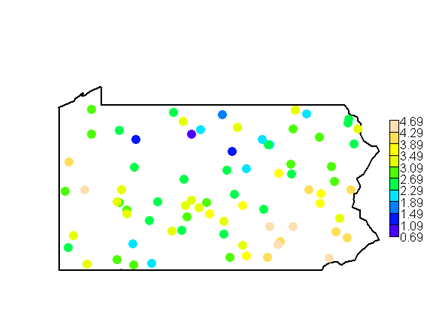
\includegraphics[height=2.75in]{figs/PA1}
\end{center}
\caption{Needs a caption}
\label{fig.PA1}
\end{figure}

We do have a measure of forest cover in the vicinity of each point which is contained in the data set (``habitat''). This was derived from a larger GIS coverage of the state (provided in the data file ``pahabdata'') which can be plotted using the spatial.plot function using the following commands
\begin{verbatim}
> map('state',regions="penn",lwd=2)
> spatial.plot(pahabdata[,2:3],pahabdata[,"dfor"],cx=2)
> map('state',regions="penn",lwd=2,add=TRUE)
\end{verbatim}


\begin{figure}
\begin{center}
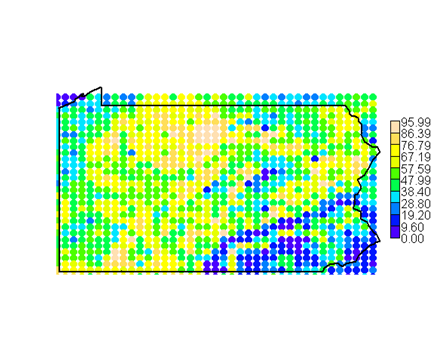
\includegraphics[height=2.75in]{figs/PA2}
\end{center}
\caption{Needs a caption}
\label{fig.PA21}
\end{figure}


We see a prominent pattern that indicates high forest coverage in the
central part of the state and low forest cover in the SE.  Inspecting
the previous figure of log-counts suggests a relationship between
counts and forest cover which is not surprising.

\subsection{Doing it in WinBUGS}
Here we demonstrate how to fit a Poisson GLM in WinBUGS using the covariate $x(i) =$ forest cover. It is advisable that $x(i)$ be standardized in most cases as this will improve mixing of the Markov chains. Recall that the data we have stored include a standardized covariate (forest cover) and so we don't have to worry about that here.  To read the BBS data into R and get things set up for WinBUGS we issue the following commands: 
\begin{verbatim}
data<-read.csv("pa-bbsdovedata-all.csv")
y<-data[,29]  # pick out 1990
notna<-!is.na(y)
y<-y[notna]
habitat<-data[notna,4]
library("R2WinBUGS")
data <- list ( "y","M","habitat")
\end{verbatim}
Now we write out the Poisson model specification in WinBUGS pseudo-code, provide initial values, identify parameters to be monitored and then execute WinBUGS:
\begin{verbatim}
cat("
model {
    for (i in 1:M){
      y[i]~dpois(lam[i])
      log(lam[i])<- beta0+beta1*habitat[i]
     }
 beta0~dunif(-5,5)
 beta1~dunif(-5,5)
}
",file="PoissonGLM.txt")

inits <- function()  list ( beta0=rnorm(1),beta1=rnorm(1))
parameters <- c("beta0","beta1")
out<-bugs (data, inits, parameters, "PoissonGLM.txt", n.thin=2, n.chains=2, n.burnin=2000,n.iter=6000,debug=TRUE,working.dir=getwd())
\end{verbatim}

{\bf Remarks:} (1) Note the close correspondence in how the model is specified here compared with the normal regression model previously. As an exercise you should discuss the specific differences between the BUGS model specifications for the normal and Poisson models.
\begin{verbatim}
> print(out,digits=3)
Inference for Bugs model at 
``PoissonGLM.txt'', fit using WinBUGS,
 2 chains, each with 4000 iterations (first 1000 discarded), n.thin = 2
 n.sims = 3000 iterations saved
             mean     sd     2.5%      25%      50%      75%    97.5%  Rhat n.eff
beta0       3.151  0.025    3.102    3.135    3.151    3.168    3.199 1.001  2300
beta1      -0.498  0.021   -0.539   -0.512   -0.498   -0.484   -0.457 1.001  3000
fit       869.930 19.856  835.500  855.700  868.600  881.900  913.602 1.002  1600
fitnew     76.709 12.519   54.098   68.107   76.215   84.510  102.602 1.001  3000
deviance 1116.605  2.014 1115.000 1115.000 1116.000 1117.000 1122.000
1.001  3000
\end{verbatim}


We might wonder whether this model provides an adequate fit to our data.  To evaluate that, we used a Bayesian p-value analysis with fit statistic based on the Freeman-Tukey residual by replacing the model specification above with this:

\begin{verbatim}
cat("
model {
    for (i in 1:M){
      y[i]~dpois(lam[i])
      log(lam[i])<- beta0+beta1*habitat[i]
      d[i]<-  pow(pow(y[i],0.5)-pow(lam[i],0.5),2)   #

      ynew[i]~dpois(lam[i])
      dnew[i]<-pow( pow(ynew[i],0.5)-pow(lam[i],0.5),2)

     }
 fit<-sum(d[])
 fitnew<-sum(dnew[])
 beta0~dunif(-5,5)
 beta1~dunif(-5,5)
}


",file="PoissonGLM.txt")
\end{verbatim}
The Bayesian p-value is the proportion of times $fitnew > fit$ which, for this data set, is 0, which was 1.0 in this case (calculation omitted). This suggests that the basic Poisson model does not fit well. 


\subsection{ Constructing your own MCMC algorithm}

It will be helpful for people to suffer through a couple examples building a custom MCMC algorithm. So, here, we build a basic one for the Poisson regression model using a Metropolis-within-Gibbs approach. First, we will assume that the two parameters have diffuse normal priors, say $[\alpha] = norm(0,100)$ and $[\beta]=norm(0,100)$.  We need to collect the relevant elements of the model which are the likelihood $[y|\alpha,\beta] = prod_{i} [y[i]|\alpha\beta] $ which is, mathematically, the product of the Poisson pmf evaluated at $y[i]$, given particular values of $\beta0$ and $\beta1$. The priors are $[\alpha]$ and $[\beta]$. We identify the full conditionals which are $[\alpha|\beta, y]$ and $[\beta|\alpha,y]$.  We use the all-purpose rule for constructing full conditionals to discover that:
\[
 [\alpha|\beta,y] propto [y|\alpha,\beta][\alpha] 
\]
\[
 [\beta|\alpha,y] propto [y|\alpha,\beta][\beta]
\]
Remember we could replace the ``propto'' with ``equals'' if we simply put $[y|\beta]$ or $[y|\alpha]$ in the denominator. But, in general, $[y|\alpha]$ or $[y|\beta]$ will be quite a pain to compute and, more importantly, it is a constant as far as the operative parameter (beta or alpha, respectively) goes so we can just as well ignore it because, recall, the MH acceptance probability will be the ratio of the ful-conditional evaluated at a candidate draw to that evaluated at the current draw. So, the denominator required to change $\propto$ to $=$ winds up canceling from the MH acceptance probability.  Here we will use the random walk candidate generator.  The ``Metropolis within Gibbs'' algorithm for a Poisson regression is remarkably simple:

%% Kimmy: test this R code out below and see what happens!

\begin{verbatim}I would break this code up into more lines and have objects called ``prior'' and ``prior.candidate'' and ``lambda'' and ``likelihood.candidate''. Annoying stuff that will make it easier for people to understand. Also, remind people that $lik*prior = exp(log(like)+log(prior))$. Lots of people have been running around in the woods for years with traps, and have forgotten math.

You could also mention that this is a random walk M-H. It would help lots of people out to see a non-symmetric proposal distribution, and the extra step needed to account for it.

# put random number seed here
out<-matrix(NA,nrow=1000,ncol=2)   # matrix to store the output
beta0<- -1                         # starting values
beta1<- -.8

# begin the MCMC loop ; do 1000 iterations
for(i in 1:1000){

# update the beta0 parameter
lik.curr<- sum(log(dpois(y,exp(beta0+beta1*habitat)))) 
prior.curr<- log(dnorm(beta0,0,100))
beta0c<-rnorm(1,beta0,.25)         # generate candidate
lik.cand<- sum(log(dpois(y,exp(beta0c+beta1*habitat))))
prior.cand<- log(dnorm(beta0c,0,100))
if(runif(1)< exp(lik.cand+prior.cand-lik.curr-prior.curr)) beta0<-beta0c

# update the beta1 parameter
lik.curr<- sum(log(dpois(y,exp(beta0+beta1*habitat)))) 
prior.curr<- log(dnorm(beta1,0,100))
beta1c<-rnorm(1,beta1,.25)
lik.cand<- sum(log(dpois(y,exp(beta0+beta1c*habitat)))) 
prior.cand<- log(dnorm(beta1c,0,100))
if(runif(1)< exp(lik.cand+prior.cand-lik.curr-prior.curr)) beta1<-beta1c
out[i,]<-c(beta0,beta1)             # save the current values
}
\end{verbatim}


\begin{figure}
\begin{center}
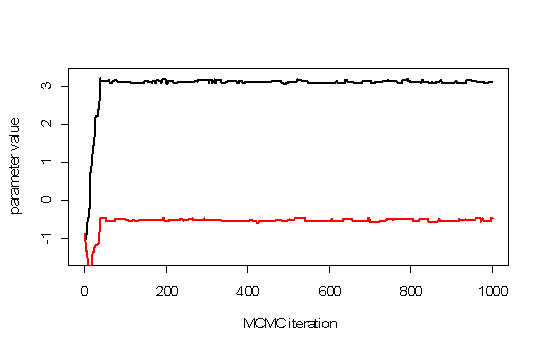
\includegraphics[height=2.75in]{figs/MCMC1}
\end{center}
\caption{Needs a caption}
\label{fig.MCMC1}
\end{figure}


Look at the output (beta0 in red, beta1 in black). You might not like the appearance of this output too much but a couple of things are evident: The Markov chains clearly stabilize - ``converge'' --  after about 100 iterations. They also appear to mix very slowly, although this is not so clear given the scale of the y-axis.
 

We decreased the variance for candidate generating distribution and
re-ran the MCMC algorithm producing the history plots below. We see
that the burn-in takes longer but it seems to mix better.


Fig. XYZ shows a longer MCMC run (10,000 total iterations) for beta1
based on discarding the first 400 samples as burn-in. The ``grassy''
look of the MCMC history is diagnostic of Markov chains that are
well-mixing.

\begin{figure}
\begin{center}
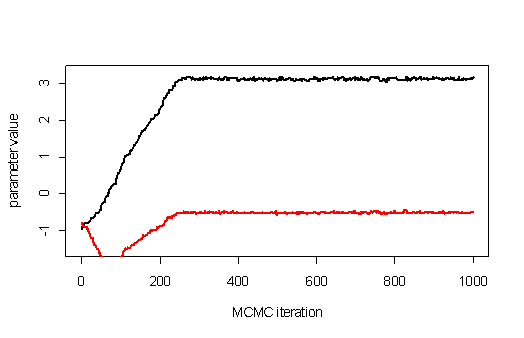
\includegraphics[height=2.75in]{figs/MCMC2}
\end{center}
\caption{Needs a caption}
\label{fig.MCMC2}
\end{figure}


\begin{figure}
\begin{center}
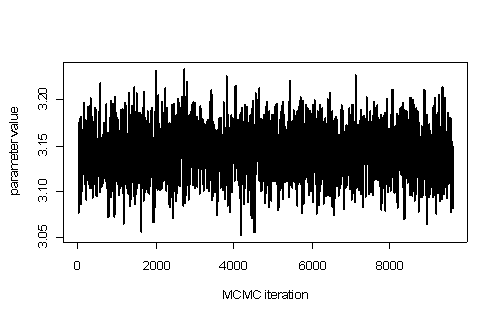
\includegraphics[height=2.75in]{figs/MCMC3}
\end{center}
\caption{nice grassy mcmc output}
\label{glms.fig.grassy}
\end{figure}

{\bf Remarks:} We used a specific set of starting values for these
simulations. It should be clear that starting values closer to the
mass of the posterior distribution might cause burn-in to occur
faster. As an exercise, evaluate that.  (2) Clearly the influence of
the proposal variance term is important. Small values lead to much
better mixing but it should be noted that values that are too small
will lead to very slow mixing. We saw that values that were too large
tended to get the parameters stuck in one spot. This suggests there is
an optimal value of the Metropolis-Hastings tuning
parameter\footnote{Defined previously?}. As an exercise you should
find that optimal value. (3) For the flat normal prior distributions
here we could leave the prior contribution out of the full conditional
evaluation since it is ``locally constant''. Note also that we have
used a different prior than in our WinBUGS model specification. As an
exercise, evaluate whether this seems to affect the result.

\section{Poisson GLM with Random Effects}

What we will be doing in most of this book is dealing with random effects in GLM-like models - models that are usually referred to as generalized linear mixed models (GLMMs).

{\bf The Log-Normal mixture:} The classical situation involves a GLM with a normally distributed random effect. The linear predictor of the Poisson model is extended simply by adding a noise term, say:
\[
 	log(\lambda(i)) = \alpha  + \beta*x(i) + \eta[i]
\]
where $\eta[i]~normal(0,\sigma2)$.  A natural alternative is to have $exp(\eta[i])/\sim\gamma(a,b)$ which would correspond to a negative binomial kind of over-dispersion whereas the normal noise has a different mean/variance relationship (the interested reader should work that out).   Choosing between such possibilities is not a topic we will get into here because it doesn't seem possible to provide general guidance on it. Anyhow, it is really amazingly simple to express this model in WinBUGS and have WinBUGS draw samples from the posterior distribution using the following code for the BBS dove counts: 
\begin{verbatim}
data<-read.csv("pa-bbsdovedata-all.csv")
locs<-data[,2:3]
habitat<-data[,4]
y<-data[,29]
notna<-!is.na(y)  # to remove missing values
y<-y[notna]
locs<-locs[notna,]
habitat<-habitat[notna]
M<-length(y)

cat("
model {
            for (i in 1:M){
               y[i]~dpois(lam[i])
               log(lam[i])<- beta0+beta1*habitat[i] + eta[i]
               eta[i] ~ dnorm(0,tau)
               }
 beta0~dunif(-5,5)
 beta1~dunif(-5,5)
 sigma~dunif(0,10)
 tau<-1/(sigma*sigma)
}
\end{verbatim}
I have removed the final several R commands which package up the data and execute WinBUGS as those commands are largely redundant with the previous demo.  The summary results are:
\begin{verbatim}
> print(out,digits=3)
Inference for Bugs model at "model.txt", fit using WinBUGS,
 2 chains, each with 5000 iterations (first 1000 discarded), n.thin = 2
 n.sims = 4000 iterations saved
            mean     sd    2.5%     25%     50%     75%   97.5%  Rhat n.eff
beta0      2.967  0.076   2.817   2.915   2.969   3.020   3.111 1.006   430
beta1     -0.518  0.073  -0.657  -0.566  -0.517  -0.470  -0.374 1.008  4000
sigma      0.598  0.059   0.491   0.556   0.594   0.634   0.725 1.004   640
tau        2.883  0.569   1.904   2.489   2.836   3.233   4.149 1.004   640
fit       19.885  3.190  14.119  17.670  19.705  21.902  26.610 1.001  4000
fitnew    20.043  3.422  14.100  17.630  19.770  22.292  27.360 1.001  4000
deviance 446.255 12.290 424.000 437.700 445.600 454.100 472.302 1.001  4000

For each parameter, n.eff is a crude measure of effective sample size,
and Rhat is the potential scale reduction factor (at convergence, Rhat=1).

DIC info (using the rule, pD = Dbar-Dhat)
pD = 66.0 and DIC = 512.2
DIC is an estimate of expected predictive error (lower deviance is better).
> 

\end{verbatim}

The Bayesian p-value for this model is
\begin{verbatim}
> mean(out$sims.list$fit>out$sims.list$fitnew)
[1] 0.473
>
\end{verbatim}
indicating a pretty good fit. Given the site-level random effect, it
would be surprising for this model to not fit! One thing we notice is
that the posterior standard deviations of the regression parameters
are much higher, a result of the excess variation. (we would also
notice much less precise predictions of hypothetical new
observations).


\section{Binomial GLMs}

Another class of statistical models that are very important in ecology are binomial models. We use binomial models for count data whenever the observations are counts or frequencies and it is natural to condition on a ``sample size'' - the maximum frequency possible in a sample, say $K$ (i.e., $K$ is known). The random variable, $y/le K$, is then the frequency of occurrences out of $K$. The parameter of the binomial models is $p$, often called ``success probability'' which is related to the expected value of $y$ by $E[y] = pK$. Binomial GLMs or binomial regression models are often referred to as logistic regression, but that term really only applies when the logistic link is used to model the relationship between $p$ and covariates (see below).

One of the most typical Binomial GLMs occurs when the sample size
equals 1 and the outcome, $y$, is ``presence'' ($y=1$) or ``absence''
($y=0$) of a species. This is a classical ``species distribution''
modeling situation. A special situation occurs when presence/absence
is observed with error \citep{mackenzie_etal:2002,
  mackenzie_etal:2006, kery_etal:2010}. In that case, $K>1$ samples
are usually required in order to estimate model parameters
effectively. In standard binomial regression problems the sample size
is fixed by design but interesting models also arise when the sample
size is itself a random variable. These are the N-mixture models
\citep{royle:2004, kery_etal:2005, royle_dorazio:2008, kery:2010}
ch. 22) and related models (in this case, $N$ being the sample size
which we labeled K above). This is actually a little bit confusing
because the binomial index is usually referred to as ``sample size''
but in this context N is actually a ``population size''.  A useful
situation in which the binomial sample size is ``fixed'' is closed
population capture-recapture models in which a population of
individuals is sampled $K$ times.  The number of times each individual
is encountered is a binomial outcome with parameter - encounter
probability - $p$, based on a sample of size $K$.  We consider such
models in the following chapter.


\subsection{Binomial regression}

 In binomial models, covariates are modeled on a suitable transformation (the link function) of the binomial success probability, $p$.  Let  $x_{i}$ denote some measured covariate for sample unit $i$ and let $p_{i}$ be the success probability for unit i.  The standard choice is the ``logit'' link function which is:
\[
log(p[i]/(1-p[i])) = \alpha + \beta*x[i]
\]
with inverse ``expit''
\[
p[i] = expit(\alpha + \beta*x[i]) = exp(\alpha + \beta*x[i])/(1 + exp(\alpha + \beta*x[i])) 
\]
There are many other possible link functions. However, ecologists seem
to blindly adopt the logit link function without question to such an
extent that you are likely to be questioned by referees and associate
editors if you use some alternative link (unless you are doing species
distribution modeling, in which case any explicit link function will
be questioned by some referees).  We sometimes use the ``complementary
log-log'' (= ``cloglog'') link function in ecological applications
because it can often be justified based on subject-matter
considerations (\citet{royle_dorazio:2008}; section XYZ) or natural
scaling relationships germane to the problem.  For example, the
cloglog link arises as the ``probability of a count greater than 0''
under a Poisson model. That is, $\Pr(y>0) = 1-exp(- \lambda)$ in which case
\[
cloglog(p) =log(- log(1-p)) = log(\lambda)
\]
So that if you have covariates in your linear predictor for $E[y]$ under a Poisson model then they are linear on the complementary log-log link of p. We will use the cloglog link in some analyses of SCR models in Chapter 4 and elsewhere.  

A natural situation in which the cloglog link arises is modeling occupancy in which $N \sim Poisson(A*\lambda)$ and you have site area, A, measured for every sample. In this case the probability that the site is occupied, psi, is related to area on the cloglog scale. i.e.,
\[
 cloglog(\psi) = log(A) + log(\lambda).
\]
There seems to be perennial debate over whether site area should be a
covariate on ``detection'' or ``occupancy'' and the above argument
suggests the latter.


\subsection{ Example: Waterfowl Banding Data}

It would be easy to consider a standard ``distribution modeling''
application where $K=1$ and the outcome is occurrence ($y=1$) or not
($y=0$) of some species. Such examples abound in books (e.g.,
\citet{royle_dorazio:2008}, ch. 3; \citet{kery:2010}, chapter 21 XYZ?;
\citet{kery_schaub:2011}, chapter XYZ) and in the literature (see
\citet{kery_etal:2010}; \citet{kery_etal:2010} XYZ).  Instead, we will consider an example involving band returns of waterfowl which were analyzed by Royle and Dubovsky (200X)\footnote{not happy about this example. Anyone got a better one?}.  

For these data, $y[i]$ is the number of waterfowl bands recovered out of $B[i]$ birds banded at some location $s[i]$. In this case $B[i]$ is fixed. Thinking about recovery rate as being proportional to harvest rate, we wanted to explore geographic gradients in recovery rate resulting from variability in harvest pressure experienced by populations depending on their migration ecology. As such, we fit a basic binomial GLM with a linear response to geographic coordinates (including an interaction term). The data are provided on the web supplement along with an R script to do the post-processing. Here we just provide the part of the script for creating the model and calling WinBUGS:

\begin{verbatim}
sink("model.txt")
cat("
model {
 for(t in 1:5){
    for (i in 1:nobs){
       m[i,t] ~ dbin(p[i,t], R[i,t])
       logit(p[i,t]) <- alpha0[t] + alpha1*X[i,1] + alpha2*X[i,2] + alpha3*X[i,1]*X[i,2]
     }
}
	alpha1~dnorm(0,.001)
	alpha2~dnorm(0,.001)
	alpha3~dnorm(0,.001)
	for(t in 1:5){
 	alpha0[t] ~ dnorm(0,.001)  
 }
}
",fill=TRUE)
sink()

data <- list('R', 'm', 'nobs','X')
inits <- 	function(){
list(alpha0=rnorm(5),alpha1=0,alpha2=0,alpha3=0)
}
parms <- list('alpha0','alpha1','alpha2','alpha3')
out <- bugs(data,inits, parms,"model.txt",n.chains=3,
 					n.iter=2000,n.burnin=1000,
					n.thin=2, debug=TRUE)
\end{verbatim}

Posterior summaries of model parameters are as follows:

\begin{verbatim}
Inference for Bugs model at "model.txt", fit using WinBUGS,
 3 chains, each with 2000 iterations (first 1000 discarded), n.thin = 2
 n.sims = 1500 iterations saved
              mean    sd     2.5%      25%      50%      75%    97.5%  Rhat n.eff
alpha0[1]   -2.346 0.036   -2.417   -2.370   -2.346   -2.323   -2.277 1.001  1500
alpha0[2]   -2.356 0.032   -2.420   -2.379   -2.356   -2.335   -2.292 1.001  1500
alpha0[3]   -2.220 0.035   -2.291   -2.244   -2.219   -2.197   -2.153 1.001  1500
alpha0[4]   -2.144 0.039   -2.225   -2.169   -2.143   -2.116   -2.068 1.000  1500
alpha0[5]   -1.925 0.034   -1.990   -1.949   -1.924   -1.901   -1.856 1.004   570
alpha1      -0.023 0.003   -0.028   -0.025   -0.023   -0.022   -0.018 1.001  1500
alpha2       0.020 0.006    0.009    0.016    0.020    0.024    0.031 1.001  1500
alpha3       0.000 0.001   -0.002   -0.001    0.000    0.000    0.002 1.001  1500
deviance  1716.001 4.091 1710.000 1713.000 1715.000 1718.000 1726.000 1.001  1500

For each parameter, n.eff is a crude measure of effective sample size,
and Rhat is the potential scale reduction factor (at convergence, Rhat=1).

DIC info (using the rule, pD = Dbar-Dhat)
pD = 7.9 and DIC = 1723.9
DIC is an estimate of expected predictive error (lower deviance is better).
\end{verbatim}

The basic result suggests a negative east-west gradient and a positive south to north gradient but no interaction. A map of the response surface is given below. We could use DIC to do some model selection - i.e., try models without the interaction term, or models with a quadratic term, or with a constant intercept, etc., but we don't pursue that here. We did an MCMC run where we saved the binomial parameter p and computed the Bayesian p-value [double use of ``p'' here is confusing!] using a fit statistic based on the Freeman-Tukey statistic (see Section XXX above). The result indicates that the linear response surface model does not provide an adequate fit of the data. The reader should contemplate whether this invalidates the basic interpretation of the result.


\begin{figure}
\begin{center}
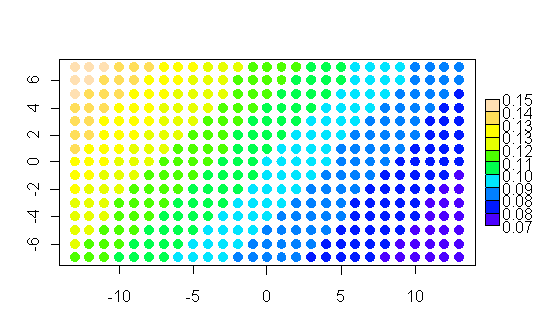
\includegraphics[height=2.75in]{figs/responsesurface}
\end{center}
\caption{Needs a caption}
\label{fig.responsesurface}
\end{figure}

\section{Stuff on hierarchical models here?}

\section{ Summary and Outlook}


GLMs and GLMMs are the most useful statistical methods in all of ecology. The principles and procedures underlying these methods are relevant to nearly all modeling and analysis problems in every branch of ecology. Moreover, understanding how to analyze these models is crucial in a huge number of diverse problems. If you understand and can conduct classical likelihood and Bayesian analysis of Poisson and binomial GLM(M)s, then you will be successful analyzing and understanding more complex classes of models that arise.We will see shortly that spatial capture-recapture models are just a type of GLMM (i.e., a GLM with a random effect) and thus having a basic understanding of the conceptual origins and formulation of GLMs and their analysis is extremely useful. We note that GLMs are routinely analyzed by likelihood methods but we have focused on Bayesian analysis here in order to develop the tools that are less familiar to most ecologists.  In particular, Bayesian analysis of GLMs with random effects (i.e., GLMMs) is relatively straightforward because the models are easy to analyze conditional on the random effect, using methods of MCMC.  Thus, we will often analyze SCR models in later chapters by MCMC, explicitly adopting a Bayesian inference framework.

In that regard, BUGS engines are enormously useful because they provides a straightforward way to carry out analyses by MCMC by just describing the model, and not having to worry about how to actually build MCMC algorithms.  That said, the BUGS language is more important than just to the extent that it enables one to do MCMC - it is useful as a modeling tool because it fosters understanding, in the sense that it forces you to become intimate with your model. You have to write down all of the probability assumptions, the relationships between observations and latent variables and parameters. This is really a great learning paradigm that you can grow with. Skills gained in Bayesian analysis of the GLMMs covered in this chapter will be directly transferrable and useful for the SCR models addressed subsequently. Before getting to that, however, it will be useful to talk about more basic, conventional closed population capture-recapture models and these are the topic of the next Chapter. 
